%=== CHAPTER ONE (1) ===
%=== INTRODUCTION ===

\chapter{Introduction}

\section{Background}

SLAM(Simultaneous localization and mapping) is an important component in developing mobile autonomous systems. It enable a vehicle the ability to explore and map an unknown environment, while at the same time estimating its own position in the environment, using only its sensors equipped onboard.

SLAM systems can be accomplished by both single or multiple robots. Multiple-robot SLAM or MRSLAM, offer several advantages compared to single robot SLAM, for example:
\begin{itemize}
	\item Robustness to failure of single robots,
	\item Faster environment exploration in time critical Search and Rescue(SaR) mission.
\end{itemize} 


However, Adapting SLAM technology to multiple-robot scenario brings some new changes as identified by Saeedi et al \cite{saeedi2016multiple}:
\begin{itemize}
	\item Relative Poses of Robots. The map created by each robot in MR-SLAM systems in its own reference is called the local map. It is a difficult task to merge all the local client maps created by each robot to create a globally consistent map of the environment, as the required transformation or alignment matrices that relate these maps to each other are generally unknown. 
	\item Closing Loops. Loop closure is defined as identifying a previously observed but not very recent place. Solving this problem for a multiple robot cluster requires taking advantage of all information resources from each client. In multi-robot SLAM, different events can trigger loop closure, such as direct or indirect robots encounter, when robots see the same area of features worldwide. 
	\item Communications. Multi-robot SLAM requires a medium to be highly available for data sharing between robots. It is possible to exchange information between robots via communication channels. The quality of the channels of communication depends on the environment. Communication, for example, is a challenging issue for a robots team in underwater environments, where the environment imposes limitations on data rate and bandwidth. 
\end{itemize}

Because of the limitation of the difficulties mentioned above, the development of multiple-robot SLAM is much slower than single-robot SLAM. Finding a solution to these problem will push the adaption of SLAM technology to a new level.

\begin{figure}
	\centering
	\subfigure[Input image and extracted keypoints.]{
		\begin{minipage}[t]{0.4\linewidth}
			\centering
			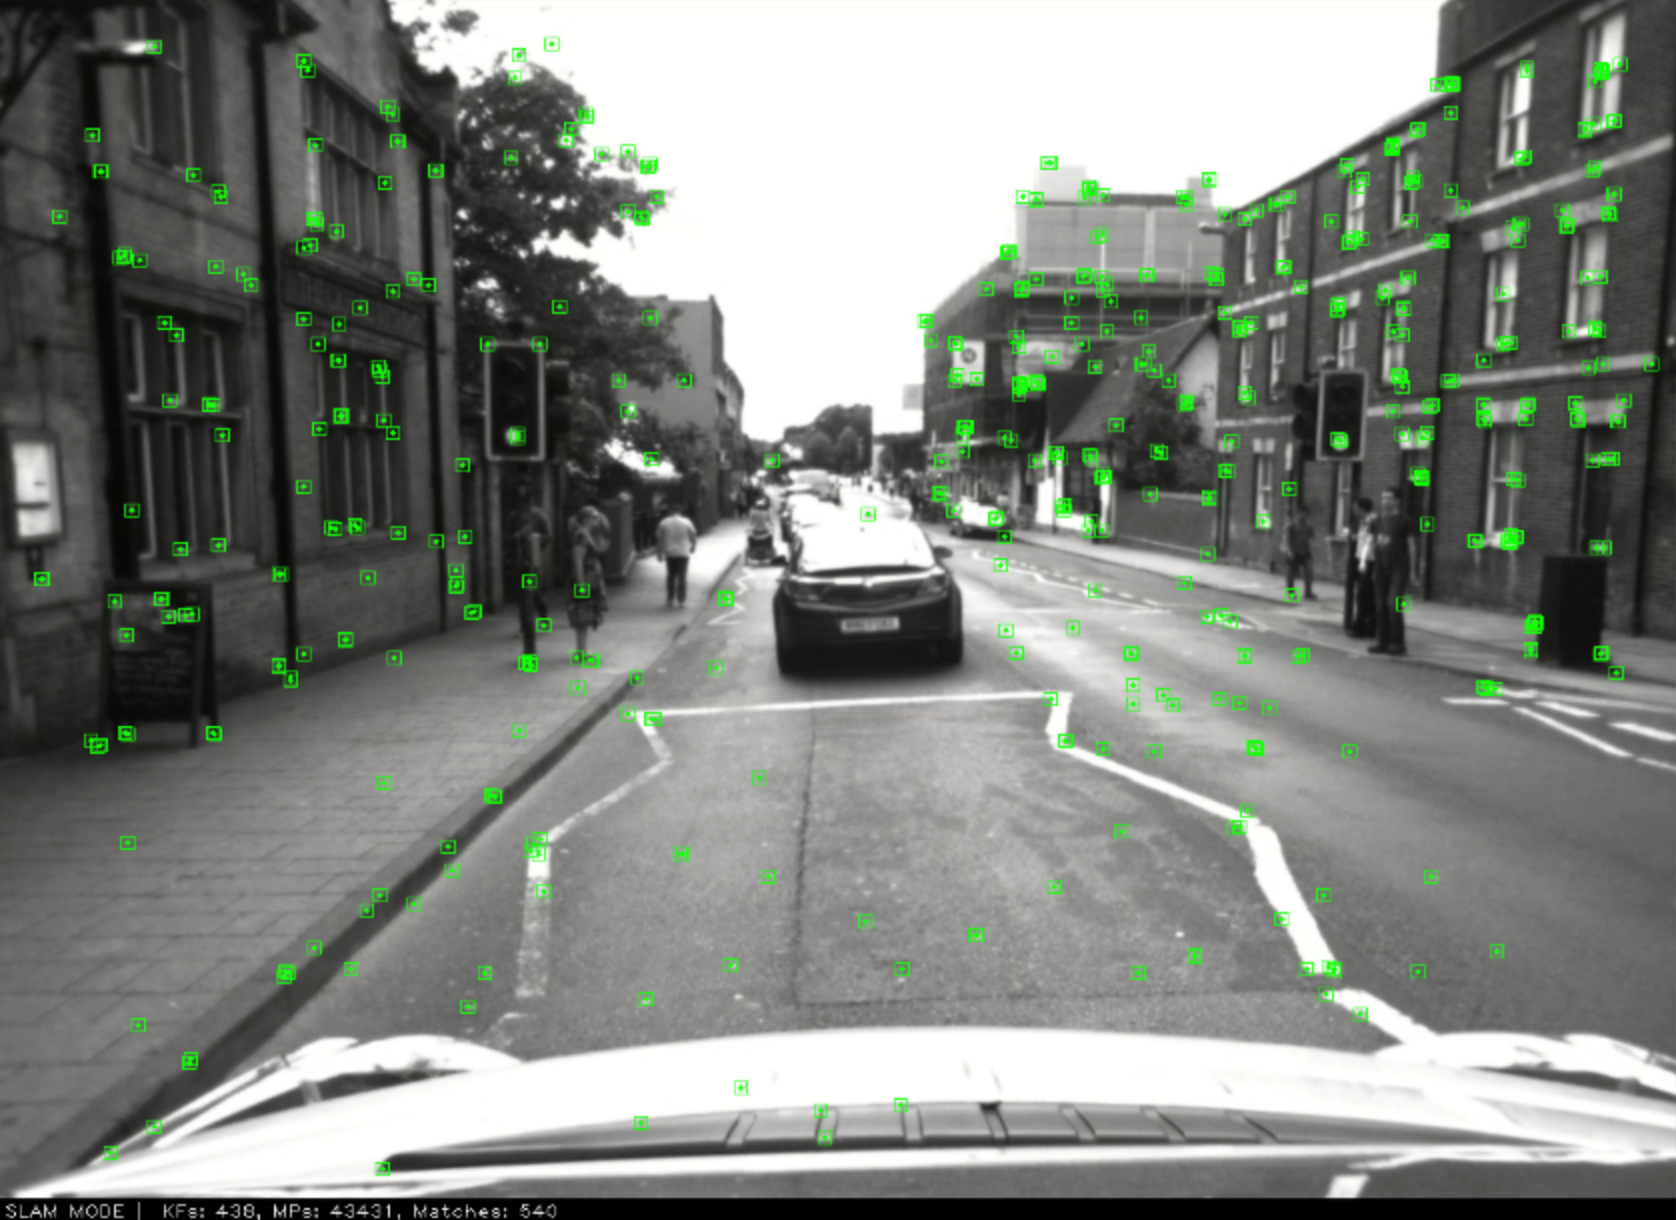
\includegraphics[width=2in]{Chapter1/introimg.eps}
			%\caption{fig1}
		\end{minipage}
	}
	\subfigure[Mapping result.]{
		\begin{minipage}[t]{0.4\linewidth}
			\centering
			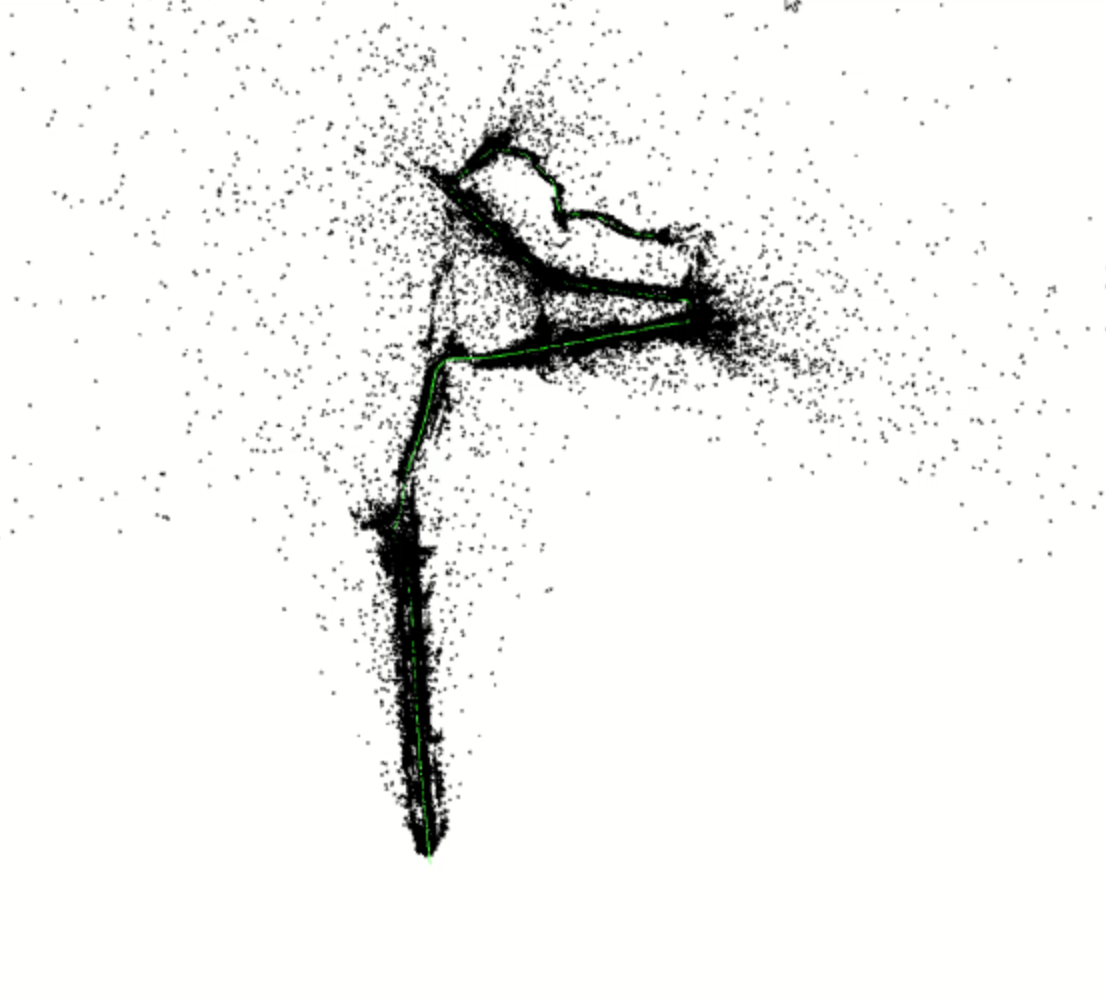
\includegraphics[width=2in]{Chapter1/intromap.eps}
			%\caption{fig2}
		\end{minipage}
	}
	\caption{A demonstration of input and mapping results of SLAM systems}
	\label{fig:backgroundslam}
\end{figure}

\section{Motivation and Objectives}

Recently, some solutions for multi-robot SLAM systems have been proposed. One of them is CORB-SLAM proposed in \cite{li2017corb}. As its clients based on ORB-SLAM, it inherits major advantages of ORB-SLAM e.g. relatively low computational cost and low cost of sensors. But in its initial work, the accuracy of its map fusion results are not evaluated in a quantitative evaluation method, while only a rough demonstration of its mapping results is given. Therefore, quantitative evaluation of CORB-SLAM with mapping results of single-robot ORB-SLAM system and CORB-SLAM clients given for comparison can help understand the performance of this multi-robot slam algorithm and assess the feasibility of its potential applications.

Another critical requirement of applications of multi-robot slam algorithms is its ability to fuse sub maps under different illumination conditions and season, which is named as long-term application circumstances. Illumination variance method proposed in \cite{maddern2014illumination}  with advantages of easy implement and low computational cost, may be able to help CORB-SLAM to deal with illumination and season changes. Therefore related experiments are undertaken in this work in order to find a effective way to combine CORB-SLAM with illumination variance.

\section{Major contribution of the Dissertation}
\begin{enumerate}[1.]
	\item Evaluation of CORB-SLAM on several datasets with quantitative trajectory evaluation results provided.
	\item Experiment of combination of CORB-SLAM with illumination variance algorithm to test whether illumination variance method is suitable to enhance ability of CORB-SLAM to deal with illumination changes.
\end{enumerate}

\section{Organisation of the Dissertation}
This dissertation is organised into several chapters:
\begin{enumerate}[1.]
	\item Chapter 2 briefly outlines the development of visual SLAM technique. Firstly, the classic structure of visual SLAM system is introduced, and the critical algorithms involved are elaborated, so as the classifications of visual SLAM systems. Then two main algorithms involved in this work, ORB-SLAM and CORB-SLAM, are demonstrated. This chapter also explores prior work in shade dealing algorithms required to implement long-term SLAM.
	
	\item Chapter 3 explains the methodology used in this dissertation to evaluate map fusion performance of CORB-SLAM, and how to combine illumination variance method with CORB-SLAM system to test if illumination variance can be utilized to enhance the ability of CORB-SLAM to deal with illumination changes.
	
	\item Chapter 4 shows the results of 
	
	\begin{inparaenum}[(a)]
		\item the evaluation of CORB-SLAM on selected 2 datasets including 
		\begin{inparaenum}[(i)]
			\item KITTI Visual Odometry Dataset \cite{Geiger2012CVPR},
			\item NTU Dataset \cite{zhang2018two},
		\end{inparaenum}
	
		\item the evaluation of CORB-SLAM combined with illumination variance on Oxford RobotCar Dataset \cite{maddern20171}.
		\end{inparaenum}
		
	\item Chapter 5 analysis the results demonstrated in chapter 4 in detail, discussing the improvement and the disadvantages.
	
	\item Chapter 6 concludes the work done in this dissertation, and comments on some limitation and drawbacks of algorithms used in this work, which future work need focus on.  

\end{enumerate}


%=== END OF CHAPTER ONE ===
\newpage


